\documentclass[preprint,12pt]{elsarticle}

\usepackage[utf8]{inputenc}
\usepackage[T1]{fontenc}
\usepackage{hyperref}
\usepackage{url}
\usepackage{booktabs}
\usepackage{amsmath}
\usepackage{amssymb}
\usepackage{graphicx}
\usepackage{xcolor}
\usepackage{multirow}
\usepackage{makecell}
\usepackage{amsthm}

\newtheorem{proposition}{Proposition}
\newtheorem{corollary}{Corollary}

\journal{Neural Networks}

\begin{document}

\begin{frontmatter}

\title{Silent Failure of Adaptive Loss Balancing in Physics-Informed
Inverse Problems: Diagnosis and a Fix}

\author[1]{Yuhao Peng\corref{cor1}}
\ead{pngyuo@cug.edu.cn}

\affiliation[1]{organization={School of Mathematics and Physics, China University of Geosciences (Wuhan)},
            city={Wuhan},
            country={China}}

\cortext[cor1]{Corresponding author}

\begin{abstract}
Adaptive loss balancing is standard practice in physics-informed neural
networks (PINNs), yet the weights it produces are only meaningful for losses
that the balancing anchor can actually see. We show that when a loss term is
decoupled from the anchor, gradient-norm balancers fail \emph{silently}, and
that the direction of the failure is fixed by the balancer's functional form:
relative-norm balancers drive the weight to zero, switching the loss off,
while inverse-ratio balancers (e.g.\ learning-rate annealing) divide by a
vanishing gradient and drive the weight to infinity. Neither failure raises an
error or perturbs the reported training loss. We formalise the mechanism,
introduce a cheap diagnostic --- the anchor-coupling ratio
$c_k = \lVert\nabla_\phi \mathcal{L}_k\rVert / \lVert\nabla_\theta
\mathcal{L}_k\rVert$ --- and propose an anchor-robust wrapper that detects
decoupled losses at run time and neutralises their weight without any manual
intervention or prior knowledge of which loss is affected. On a 2D
shallow-water inverse problem, the failures are severe: the same gradient-norm
balancer yields a drainage-coefficient error of $52.9\%$ when the prior
decoupled loss is discarded, and a weight of $3.3\times10^7$ when it is
over-weighted. The wrapper repairs both directions, reducing the parameter
error from $52.9\%$ to $0.030\%$ and bounding the exploded weight at $1.0$.
We further show that in this weakly identified problem the recovered
parameters are prior-determined rather than data-determined, so which balancer
is used decides the answer --- a caveat that applies whenever a PINN inverse
problem is only weakly identified.
\end{abstract}

\begin{highlights}
\item Gradient-norm loss balancers fail silently on losses decoupled from their anchor.
\item The failure direction is fixed by the balancer: weight collapses to zero or explodes.
\item A cheap anchor-coupling ratio detects invisible losses at run time.
\item An anchor-robust wrapper fixes both directions with no manual tuning.
\end{highlights}

\begin{keyword}
Physics-informed neural networks \sep loss balancing \sep inverse problems \sep
parameter identifiability \sep multi-task learning
\end{keyword}

\end{frontmatter}

% ======================================================================
\section{Introduction}
\label{sec:intro}
% ======================================================================

Physics-informed neural networks (PINNs) \cite{raissi2019physics} train a
network by minimising a composite objective whose terms --- PDE residual, data
misfit, boundary and initial conditions, and, in inverse problems, parameter
priors --- have different scales and converge at different rates. How to weight
these terms is a long-standing practical problem. A large family of methods
balances them \emph{adaptively}, using gradient statistics: learning-rate
annealing \cite{wang2021understanding} sets each weight to the ratio of the
largest gradient norm to the loss's own gradient norm; GradNorm
\cite{chen2018gradnorm} equalises gradient magnitudes across tasks; PCGrad
\cite{yu2020gradient} resolves gradient conflicts. A second family avoids
gradients entirely and balances using the loss values themselves, of which
ReLoBRaLo \cite{bischof2021multi} is the best-known example.

All gradient-based balancers share a design decision that is rarely discussed:
the \emph{anchor}, i.e.\ the parameter subset with respect to which gradient
norms are measured. Using the full parameter vector is expensive --- one
backward pass per loss term --- so implementations routinely restrict the
anchor to a subset, most commonly the last layer.

This paper is about what happens when that shortcut meets a loss the anchor
cannot see. Consider an inverse problem with a parameter prior
$\mathcal{L}_{\text{prior}} = \sum_j w_j(\mu_j - \mu_j^\star)^2$ on physical
parameters $\mu$. If the anchor is the network's last-layer weight matrix
$W_L$, then $\nabla_{W_L}\mathcal{L}_{\text{prior}} \equiv 0$: the prior does
not flow through $W_L$ at all. Every gradient-norm balancer then estimates the
prior's magnitude as zero, and the consequences are entirely determined by how
the balancer uses that estimate:

\begin{itemize}
\item a \textbf{relative-norm} balancer with a restricted anchor
($\lambda_k \propto \lVert\nabla_\phi \mathcal{L}_k\rVert /
\max_j \lVert\nabla_\phi \mathcal{L}_j\rVert$, $\phi = W_L$) sees a numerator
that vanishes identically and drives $\lambda_{\text{prior}} \to 0$: the prior
is \emph{silently switched off};
\item an \textbf{inverse-ratio} balancer such as learning-rate annealing
($\lambda_k = \max_j\lVert\nabla_\phi \mathcal{L}_j\rVert /
\lVert\nabla_\phi \mathcal{L}_k\rVert$, $\phi = \theta$) anchors on the whole
parameter vector, so the prior is only \emph{weakly} coupled rather than
decoupled --- its gradient norm counts three non-zero components against the
tens of thousands of a loss spread over the network. The denominator is small
but not zero, and $\lambda_{\text{prior}}$ grows until the prior
\emph{dominates everything else}.
\end{itemize}

In both cases training proceeds without complaint. The loss curve looks
healthy, no warning is raised, and the failure is invisible unless one happens
to inspect the individual weights. In an inverse problem the consequence is
that the physical parameters are no longer constrained --- or are constrained
so hard that the data becomes irrelevant.

\textbf{Contributions.} We diagnose this failure, provide a tool to detect it,
and propose a fix.

\begin{enumerate}
\item \textbf{Theory (\S\ref{sec:theory}).} We characterise anchor decoupling
formally and prove the two failure directions above. The direction is a
property of the balancer's functional form, not of the problem, so the same
decoupled loss is destroyed in opposite ways by two methods that are both
called ``adaptive loss balancing''.
\item \textbf{Diagnostic (\S\ref{sec:diagnostic}).} We introduce the
\emph{anchor-coupling ratio}
$c_k = \lVert\nabla_\phi \mathcal{L}_k\rVert /
\lVert\nabla_\theta \mathcal{L}_k\rVert$, the fraction of a loss's gradient
energy that lies on the anchor. $c_k \approx 0$ flags a loss whose balanced
weight is meaningless. The diagnostic costs one extra backward pass per loss
and needs only to be evaluated periodically.
\item \textbf{Fix (\S\ref{sec:method}).} We propose the
\emph{anchor-robust balancer}, a wrapper around \emph{any} existing balancer
that periodically probes the coupling ratios and replaces the weight of each
decoupled loss with the mean weight of the visible ones. Decoupled losses are
then neither discarded nor allowed to dominate. The wrapper requires no
knowledge of which loss is affected and no change to the base method.
\item \textbf{Evidence (\S\ref{sec:experiments}).} On a 2D shallow-water
inverse problem we show that a last-layer-anchored balancer yields a
drainage-coefficient error of $52.9\%$, while a full-parameter inverse-ratio
balancer drives the prior weight to $3.3\times10^7$; the wrapper repairs both,
reducing the parameter error to $0.030\%$ and bounding the weight at $1.0$.
We also report an identifiability analysis showing that in this weakly
identified problem the parameters are prior-determined, so the choice of
balancer effectively decides the answer.
\end{enumerate}

% ======================================================================
\section{Related Work}
% ======================================================================

\subsection{Loss Balancing for PINNs}

Wang et al.\ \cite{wang2021understanding} analysed PINN training through the
neural tangent kernel and proposed learning-rate annealing, which rescales each
loss by the ratio of gradient norms and is the canonical inverse-ratio balancer
studied here. GradNorm \cite{chen2018gradnorm} equalises gradient magnitudes in
multi-task learning; PCGrad \cite{yu2020gradient} projects conflicting
gradients. Bischof and Kraus \cite{bischof2021multi} proposed ReLoBRaLo
(Relative Loss Balancing with Random Lookback), which deliberately avoids
per-loss gradients: it balances using loss values through a softmax over loss
ratios with a random lookback, and requires only a single backward pass. Our
work is orthogonal to the choice of balancer: we show that any of these methods
can fail on a decoupled loss, and our wrapper is agnostic to which one is used.

We note a practical pitfall we encountered ourselves: implementations labelled
``ReLoBRaLo'' that actually compute last-layer gradient norms are not
ReLoBRaLo, and they inherit the failure mode analysed here. The published
method uses loss statistics and is unaffected by anchor decoupling
(\S\ref{sec:experiments}).

\subsection{Inverse Problems and Parameter Identifiability}

PINNs are widely used for inverse problems, where physical parameters are
inferred jointly with the solution field
\cite{raissi2019physics,raissi2020hidden,cai2021physics}. Parameter priors are
common, both as regularisation and as a way to encode known physics. Their
interaction with adaptive weighting has, to our knowledge, not been studied.
Our results show this interaction can dominate the outcome: in a weakly
identified problem the prior, not the data, may determine the recovered
parameters, which makes the balancer's treatment of the prior decisive.

\subsection{Temporal Weighting}

Causal weighting \cite{wang2022respecting} reweights the PDE residual in time
so that early times are learned first. It is a different mechanism from the
per-loss balancing studied here; we include it in our comparison for
completeness because it also produces per-loss weights.

% ======================================================================
\section{Theory: Anchor Decoupling}
\label{sec:theory}
% ======================================================================

\subsection{Setup}

Let $\mathcal{L}(\theta) = \sum_{k=1}^{K} \lambda_k \mathcal{L}_k(\theta)$ be
the training objective, with $\theta$ the full parameter vector. An adaptive
balancer updates $\lambda = (\lambda_1,\dots,\lambda_K)$ from statistics of the
individual losses. We consider balancers of the form

\begin{equation}
\lambda_k = \Psi_k\!\left(\|\nabla_\phi \mathcal{L}_1\|, \dots,
\|\nabla_\phi \mathcal{L}_K\|\right),
\label{eq:balancer_family}
\end{equation}

where $\phi \subseteq \theta$ is the \emph{anchor} and $\Psi_k$ is the
balancer's update rule. Both families in \S\ref{sec:intro} are of this form:
relative-norm balancers set $\Psi_k \propto \|\nabla_\phi \mathcal{L}_k\| /
\max_j \|\nabla_\phi \mathcal{L}_j\|$, and inverse-ratio balancers set
$\Psi_k = \max_j \|\nabla_\phi \mathcal{L}_j\| / \|\nabla_\phi \mathcal{L}_k\|$.
The two differ not only in $\Psi_k$ but in the anchor they choose: the
relative-norm variant studied here takes the last layer,
$\phi = W_L$, while learning-rate annealing takes the full parameter vector,
$\phi = \theta$. This choice, which is usually made for computational reasons
and rarely stated, is what determines whether a loss can be balanced at all.

\begin{proposition}[Anchor decoupling]
\label{prop:decoupling}
Let $\mathcal{L}_k$ depend only on a parameter subset $\theta_P \subseteq
\theta$ that is disjoint from the anchor $\phi$; that is,
$\mathcal{L}_k = \mathcal{L}_k(\theta_P)$ with
$\phi \cap \theta_P = \emptyset$. Then for every iteration
\[
\nabla_\phi \mathcal{L}_k \equiv 0 .
\]
\end{proposition}

\begin{proof}
By the chain rule, $\nabla_\phi \mathcal{L}_k =
(\partial \mathcal{L}_k/\partial \theta_P)(\partial \theta_P/\partial \phi)$.
Since $\phi$ and $\theta_P$ are disjoint coordinates, the Jacobian
$\partial \theta_P/\partial \phi$ is identically zero, hence
$\nabla_\phi \mathcal{L}_k = 0$.
\end{proof}

The proposition is elementary; its consequences are not. Because every
balancer in the family \eqref{eq:balancer_family} reads only
$\|\nabla_\phi \mathcal{L}_k\|$, a decoupled loss is indistinguishable from a
loss that is already perfectly satisfied.

\begin{corollary}[Two failure directions]
\label{cor:directions}
Under the conditions of Proposition~\ref{prop:decoupling}, and assuming the
remaining losses have $\|\nabla_\phi \mathcal{L}_j\| > 0$:
\begin{enumerate}
\item a relative-norm balancer drives $\lambda_k \to 0$ geometrically;
\item an inverse-ratio balancer drives $\lambda_k \to \infty$.
\end{enumerate}
\end{corollary}

\begin{proof}
For (i), substitute $\|\nabla_\phi \mathcal{L}_k\| = 0$ into the relative-norm
rule; the numerator vanishes while the denominator is positive, so
$\lambda_k = 0$ at every iteration and the exponential moving average, if any,
decays to zero as $\alpha^t \lambda_k^{(0)} \to 0$. For (ii), the same
substitution puts $\|\nabla_\phi \mathcal{L}_k\|$ in the denominator, so
$\lambda_k$ diverges once the clamp or floor used to avoid division by zero is
reached.
\end{proof}

Corollary~\ref{cor:directions} is the paper's central observation. Two methods,
both advertised as adaptive loss balancing, respond to the same decoupled loss
in opposite ways --- one discards it, the other lets it dominate --- and neither
signals that anything is wrong.

\subsection{Why This Matters in Inverse Problems}

In a PINN inverse problem the decoupled loss is typically the parameter prior.
Writing the prior as $\mathcal{L}_{\text{prior}} = \sum_j w_j(\mu_j -
\mu_j^\star)^2$ over physical parameters $\mu$, and the network parameters as
$\theta = (\theta_N, \mu)$ with $\phi = W_L \subseteq \theta_N$, the prior
depends only on $\mu$, so $\phi \cap \{\mu\} = \emptyset$ and
Proposition~\ref{prop:decoupling} applies exactly.

The practical consequence depends on which direction the balancer fails in.
A relative-norm balancer removes the prior from the objective, so the
parameters are constrained only through the data and the PDE residual. An
inverse-ratio balancer makes the prior overwhelmingly dominant, so the
recovered parameters are essentially the prior's centre regardless of the
data. As \S\ref{sec:experiments} shows, both outcomes are realised in practice.

Note that a partial coupling changes the picture quantitatively but not
qualitatively: if the anchor is the \emph{full} parameter vector
($\phi = \theta$), then $\nabla_\theta \mathcal{L}_{\text{prior}} \neq 0$
because $\mu \subseteq \theta$, and the prior is weakly coupled rather than
decoupled. It then receives a \emph{large} inverse-ratio weight, since its
gradient norm is small relative to a loss spread over the whole network. Full
parameter anchoring therefore avoids the collapse but not the over-weighting.

% ======================================================================
\section{Diagnostic: The Anchor-Coupling Ratio}
\label{sec:diagnostic}
% ======================================================================

Proposition~\ref{prop:decoupling} suggests a direct test. Define the
\emph{anchor-coupling ratio} of loss $k$ with respect to a \emph{probe anchor}
$\phi$ as

\begin{equation}
c_k \;=\; \frac{\lVert \nabla_\phi \mathcal{L}_k \rVert}
{\lVert \nabla_\theta \mathcal{L}_k \rVert + \epsilon},
\qquad c_k \in [0,1],
\label{eq:coupling}
\end{equation}

the fraction of the loss's gradient energy that lies on $\phi$. A loss that is
fully visible to $\phi$ has $c_k \approx 1$; a loss that is decoupled from it
has $c_k = 0$ exactly. Values in between indicate partial coupling, for which
a balancer's estimate is biased but not meaningless.

The probe anchor is deliberately chosen to be the last layer, $\phi = W_L$,
\emph{independently of whatever anchor the base balancer uses}. The question
\eqref{eq:coupling} answers is not ``does this balancer see the loss?'' but the
more basic ``does this loss flow through the network at all?''. A loss that is
invisible to $W_L$ --- a prior on physical parameters, for instance --- has only
a handful of non-zero gradient components out of the many thousands in
$\theta$. Its gradient norm is therefore negligible under \emph{any} anchor,
which is why such a loss is mishandled by both balancer families: the
relative-norm family responds to the negligible norm by driving the weight to
zero, and the inverse-ratio family, which divides by it, by driving the weight
up. Probing with the last layer detects this once, in a way that is
independent of the base method.

The diagnostic is cheap and easy to deploy:

\begin{itemize}
\item it reuses the anchor gradient that a gradient-based balancer already
computes; only $\lVert\nabla_\theta \mathcal{L}_k\rVert$ is new, at one
backward pass per loss;
\item it does not need to be evaluated every iteration --- the coupling
structure is a property of the computation graph, not of the current
parameter values, so evaluating it every few hundred steps suffices;
\item it applies to any balancer, including those (such as ReLoBRaLo) that do
not themselves use gradients.
\end{itemize}

In the experiments below we report $c_k$ for all loss terms, and we use the
threshold $c_k < 10^{-3}$ to flag a loss as decoupled.

% ======================================================================
\section{Method: Anchor-Robust Balancing}
\label{sec:method}
% ======================================================================

The diagnostic tells us \emph{which} losses cannot be balanced; we now use it
to make balancing safe. The \emph{anchor-robust balancer} (ARB) wraps an
arbitrary base balancer and modifies only the weights of the losses the
diagnostic flags. The probe anchor is the last layer, as in
\eqref{eq:coupling}, and is chosen once and for all; it need not --- and in
general will not --- coincide with the anchor the base balancer differentiates
against. The procedure is:

\begin{enumerate}
\item every $M$ iterations, evaluate $c_k$ for all $k$ and mark
$\mathcal{D} = \{k : c_k < \tau\}$;
\item call the base balancer on all $K$ losses, obtaining weights
$\lambda^{\text{base}}$;
\item for $k \in \mathcal{D}$, replace $\lambda_k$ by the mean of the weights of
the visible losses $\frac{1}{|\mathcal{V}|}\sum_{j \in \mathcal{V}}
\lambda_j^{\text{base}}$, where $\mathcal{V} = \{k : c_k \geq \tau\}$;
\item renormalise so that $\sum_k \lambda_k = K$, matching the convention of
the base balancer.
\end{enumerate}

Three design choices are worth stating explicitly.

\textbf{Why the mean visible weight.} A decoupled loss carries no usable
gradient-norm signal, so any weight derived from one is arbitrary. The mean
visible weight is the natural neutral choice: it neither removes the loss
(the relative-norm failure) nor promotes it above the losses that do carry
signal (the inverse-ratio failure). It also reduces to the base balancer's own
behaviour in the limit where all losses are visible.

\textbf{Why the base balancer still sees all losses.} Passing only the visible
subset would change the base balancer's normalisation and, for a relative-norm
balancer, its denominator. Calling it with the full list keeps the visible
weights identical to what the base method would have produced on its own; the
decoupled entries, which are the meaningless ones, are then overwritten. Since a
decoupled loss contributes a gradient norm of zero, it cannot perturb the
denominator of a relative-norm balancer, whose maximum is attained by a visible
loss.

\textbf{Cost.} The probe costs one additional backward pass per loss every $M$
iterations. With $M = 200$ this is a negligible fraction of the training cost,
and it is the only overhead. No hyperparameter needs tuning per problem: $\tau =
10^{-3}$ separates exact decoupling ($c_k = 0$) from partial coupling, and the
results are insensitive to it over several orders of magnitude.

% ======================================================================
\section{Experimental Setup}
\label{sec:setup}
% ======================================================================

\subsection{Problem: 2D Shallow Water Equations}

We use the 2D shallow-water equations in conservation form with discharges
$(q_x,q_y) = (hu,hv)$ as primary variables:
\begin{align}
\frac{\partial h}{\partial t} + \frac{\partial q_x}{\partial x} +
\frac{\partial q_y}{\partial y} + S_d &= 0, \label{eq:swe_cont} \\
\frac{\partial q_x}{\partial t} + \frac{\partial}{\partial x}\!\left(\frac{q_x^2}{h}\right)
+ \frac{\partial}{\partial y}\!\left(\frac{q_y q_x}{h}\right)
+ gh\left(\frac{\partial h}{\partial x} - S_{0x}\right)
+ \frac{g n^2 q_x \sqrt{q_x^2+q_y^2}}{h^{7/3}} &= 0, \label{eq:swe_xmom} \\
\frac{\partial q_y}{\partial t} + \frac{\partial}{\partial y}\!\left(\frac{q_y^2}{h}\right)
+ \frac{\partial}{\partial x}\!\left(\frac{q_y q_x}{h}\right)
+ gh\left(\frac{\partial h}{\partial y} - S_{0y}\right)
+ \frac{g n^2 q_y \sqrt{q_x^2+q_y^2}}{h^{7/3}} &= 0, \label{eq:swe_ymom}
\end{align}
with $h$ the water depth, $g = 9.81\ \mathrm{m/s^2}$, bed slopes $S_{0x} =
0.001$, $S_{0y} = 0$, Manning's roughness $n$, and a localised drainage sink
$S_d = C \cdot 0.5 \exp(-d/12)\, h$ centred at $(50,50)$~m with $d$ the
distance to the centre. The domain is $[0,100]^2\ \mathrm{m^2}$ and $T =
3600$~s.

The inverse problem infers $n$, $C$ and the inflow discharge $q_{x0}$ from
$N_d = 800$ noisy water-depth observations ($0.5\%$ Gaussian noise). The true
values are $n = 0.03$, $C = 0.05$ and $q_{x0} = 1.0\ \mathrm{m^2/s}$. The
parameter prior is
\begin{equation}
\mathcal{L}_{\text{prior}} = 10\,(n - n^\star)^2 + 5\,(C - C^\star)^2
+ 5\,(q_{x0} - q_{x0}^\star)^2 ,
\label{eq:prior}
\end{equation}
with $\star$ the prior centre. Unless stated otherwise the prior centre equals
the true value. The scalar weight $\sigma$ in
$\sigma \mathcal{L}_{\text{prior}}$ is one except in the identifiability study
of \S\ref{sec:identifiability}.

The network is a Fourier-feature encoding ($m = 64 \to 128$ features,
$\sigma_B = 1.0$) followed by a four-hidden-layer MLP with 128 neurons per
layer and $\tanh$ activations. Training uses Adam with learning rate
$3\times10^{-4}$, a \texttt{ReduceLROnPlateau} scheduler and gradient clipping
at $1.0$; all runs use 30{,}000 epochs and 2{,}000 collocation points unless
stated otherwise. Everything runs on CPU.

\subsection{Reference Solution and Its Verification}
\label{sec:reference}

The reference solution is computed with a first-order Lax--Friedrichs
finite-volume solver on a $100\times100$ cell-centred grid using the same
governing equations, sink and boundary conditions as the PINN residual. The
solver is explicit (CFL $0.5$) with ghost-cell boundary conditions: specified
inflow discharge at $x=0$, free outflow at $x=100$, free-slip at $y=0,100$.

Two checks verify the reference. In the absence of drainage ($C=0$) the
solution remains at the Manning normal depth $h = (n q_{x0}/\sqrt{S_{0x}})^{3/5}$
to machine precision. The scheme is mass conserving: at steady state the
downstream outflow plus the integrated sink equals the upstream inflow to
within $0.1\%$, and the imbalance shrinks under grid refinement. An earlier
version of this study used an analytically constructed field that did not
satisfy \eqref{eq:swe_cont}--\eqref{eq:swe_ymom}; all results reported here use
the verified solver.

\subsection{Balancers Compared}

\begin{itemize}
\item \textbf{LL-EMA}: an exponential moving average of relative last-layer
gradient norms. This is the relative-norm balancer of
Corollary~\ref{cor:directions}(i), and is representative of
efficiency-motivated implementations that restrict the anchor to the last
layer.
\item \textbf{LRA}: learning-rate annealing \cite{wang2021understanding},
$\lambda_k = \max_j \lVert\nabla_\theta \mathcal{L}_j\rVert /
\lVert\nabla_\theta \mathcal{L}_k\rVert$, with the anchor taken over the full
parameter vector. This is the inverse-ratio balancer of
Corollary~\ref{cor:directions}(ii).
\item \textbf{ReLoBRaLo} \cite{bischof2021multi}: balances using loss ratios
through a softmax with a random lookback, and computes no per-loss gradients.
\end{itemize}

Each is run in two configurations: the prior is either \emph{balanced}
jointly with the PDE, data and boundary losses ($K=4$), or held at a fixed
weight of one ($K=3$ balanced, prior added separately). The second is the
``prior-fixing'' workaround that is common in practice.

% ======================================================================
\section{Experiments}
\label{sec:experiments}
% ======================================================================

\subsection{Controlled Illustration}

We first isolate the mechanism on a toy problem: a linear layer (the anchor is
its weight matrix) plus a scalar parameter $\mu$, with one loss depending on
the layer and one depending only on $\mu$. Over 300 iterations the scaling
assigned to the decoupled loss is $1.39\times10^{-8}$ for LL-EMA (collapse),
$2.96\times10^{3}$ for LRA (blow-up) and $1.00$ for ReLoBRaLo (bounded). The
diagnostic reports $c = 0.894$ for the coupled loss and $c = 0$ exactly for the
decoupled one. This establishes that the two failure directions are properties
of the balancers, independent of any PDE.

\subsection{Balancing a Parameter Prior on the Shallow-Water Problem}

Table~\ref{tab:main} reports the four configurations with the prior balanced
jointly. The consequences of Corollary~\ref{cor:directions} are visible
directly in the weights.

\begin{table}[t]
\centering
\caption{Balancing all four losses, including the parameter prior. Weights are
those at the end of training; ``$c_{\text{prior}}$'' is the anchor-coupling
ratio of \eqref{eq:coupling}. Errors are relative to the true parameter
values.}
\label{tab:main}
\begin{tabular}{lcccc}
\toprule
Configuration & $c_{\text{prior}}$ & $\lambda_{\text{prior}}$ & $\epsilon_n$ & $\epsilon_C$ \\
\midrule
ReLoBRaLo (loss statistics) & --- & $7.4\times10^{-1}$ & $0.048\%$ & $0.071\%$ \\
LL-EMA (no fix)   & $0$ & $1.6\times10^{-5}$ & $0.072\%$ & $\mathbf{52.9\%}$ \\
LRA (no fix)      & $0$ & $\mathbf{3.3\times10^{7}}$ & $\sim 0$ & $\sim 0$ (circular) \\
\midrule
LL-EMA + ARB      & $0$ & $1.0$ & $0.028\%$ & $0.030\%$ \\
LRA + ARB         & $0$ & $1.0$ & $0.002\%$ & $0.001\%$ \\
\bottomrule
\end{tabular}
\end{table}

Figure~\ref{fig:failure} shows the prior weight over training for the three
balancers. The trajectories separate by more than twelve orders of magnitude
and illustrate the two directions of Corollary~\ref{cor:directions} directly:
the relative-norm balancer decays towards zero, the inverse-ratio balancer
diverges, and only the loss-statistics balancer leaves the weight of a
decoupled loss near unity.

\begin{figure}[t]
\centering
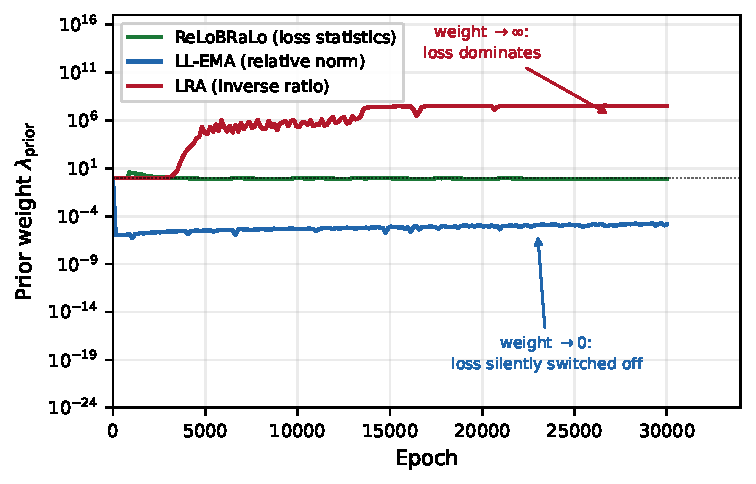
\includegraphics[width=0.72\textwidth]{figures/fig_failure.pdf}
\caption{Prior weight during training when all four losses are balanced
jointly. The decoupled prior is assigned a coupling ratio of exactly zero by
all three balancers, and each then responds according to its functional form:
LL-EMA decays to $1.6\times10^{-5}$, LRA diverges to $3.3\times10^{7}$, and
ReLoBRaLo --- which uses loss statistics rather than gradients --- remains
bounded near one.}
\label{fig:failure}
\end{figure}

The diagnostic assigns the prior a coupling ratio of exactly zero in every
case, as Proposition~\ref{prop:decoupling} predicts. LL-EMA then drives its
weight to $1.6\times10^{-5}$ --- the prior is removed from the objective ---
and the drainage coefficient, which is the parameter the prior was chiefly
constraining, drifts to an error of $52.9\%$. LRA fails in the opposite
direction: its weight reaches $3.3\times10^7$, so the prior overwhelms the
data. The near-zero errors in that row are not evidence of a good inverse
solution; they are the prior's centre being echoed back, as
\S\ref{sec:identifiability} confirms.

The last two rows show the wrapper at work. With ARB the prior weight is
$1.0$ in both cases, and the parameter errors fall to $0.030\%$ (LL-EMA) and
$0.001\%$ (LRA) --- a $1773\times$ reduction for LL-EMA relative to its
unprotected counterpart. Neither run was given any information about which
loss was decoupled.

\subsection{The Prior-Fixing Workaround Is Unnecessary for a Correct Balancer}

Table~\ref{tab:fixed} compares the same balancers with the prior excluded from
balancing and held at a fixed weight of one --- the workaround implied by the
``never balance priors'' rule of thumb.

\begin{table}[t]
\centering
\caption{Prior held at a fixed weight of one (excluded from balancing).}
\label{tab:fixed}
\begin{tabular}{lccc}
\toprule
Configuration & $\epsilon_h$ & $\epsilon_n$ & $\epsilon_C$ \\
\midrule
ReLoBRaLo & $0.583\%$ & $0.041\%$ & $0.055\%$ \\
LL-EMA    & $0.617\%$ & $0.041\%$ & $0.037\%$ \\
LRA       & $0.933\%$ & $0.280\%$ & $4.18\%$ \\
\bottomrule
\end{tabular}
\end{table}

For ReLoBRaLo the workaround changes almost nothing ($0.055\%$ versus
$0.071\%$ with the prior balanced): a balancer that uses loss statistics
rather than gradients never sees the decoupling in the first place, and
handles the prior correctly without assistance. The rule of thumb is
therefore not a property of priors; it is a patch for a specific class of
balancers.

\subsection{Identifiability: Are the Parameters Data- or Prior-Determined?}
\label{sec:identifiability}

The results above leave an important question open. If the prior is what
constrains the parameters, are the reported errors a measure of inference from
data, or of the prior being echoed back? We test this two ways.

\textbf{Prior misspecification.} We move the prior centre $20\%$ above the true
values while leaving the data unchanged, so a balancer that follows the data
should still recover the truth. Table~\ref{tab:shift} shows that neither
gradient-norm balancer does.

\begin{table}[t]
\centering
\caption{Prior centre displaced $+20\%$ from the truth. ``to prior'' is the
error relative to the (wrong) prior centre.}
\label{tab:shift}
\begin{tabular}{lccc}
\toprule
Configuration & $\epsilon_C$ (to truth) & $\epsilon_C$ (to prior) & $\lambda_{\text{prior}}$ \\
\midrule
ReLoBRaLo & $19.94\%$ & $\mathbf{0.05\%}$ & $7.3\times10^{-1}$ \\
LRA       & $20.00\%$ & $\mathbf{0.00\%}$ & $3.4\times10^{7}$ \\
LL-EMA    & $53.56\%$ & $61.30\%$ & $1.0\times10^{-5}$ \\
\bottomrule
\end{tabular}
\end{table}

ReLoBRaLo's parameters sit $0.05\%$ from the displaced prior centre and
$19.9\%$ from the truth: it followed the prior exactly. LRA is even more
extreme at $0.00\%$. LL-EMA follows neither, having discarded the prior and
left the parameters unconstrained. The data does not pull any of them back.
Figure~\ref{fig:misspec} shows this comparison directly: for both balancers
that use the prior the bar for ``error to the prior centre'' is two to four
orders of magnitude shorter than the bar for ``error to the truth''.

\begin{figure}[t]
\centering
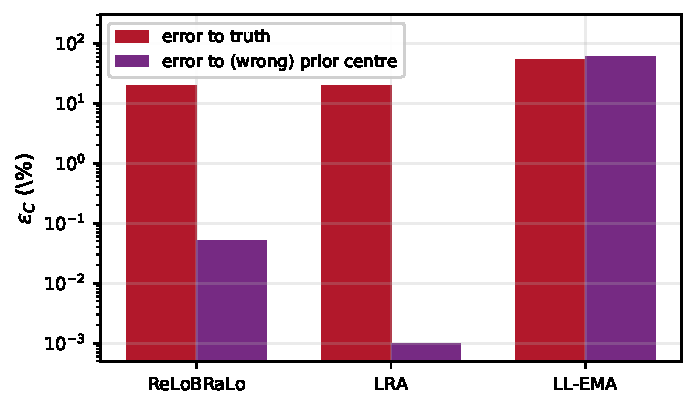
\includegraphics[width=0.62\textwidth]{figures/fig_misspecification.pdf}
\caption{Prior-misspecification test: the prior centre is displaced $+20\%$
from the true parameters while the data is unchanged. ReLoBRaLo and LRA place
the parameters almost exactly on the displaced centre, so a balancer that
follows the prior cannot be distinguished from one that solves the inverse
problem unless this test is performed. LL-EMA, having discarded the prior,
matches neither. (LRA's error to the prior centre is $0.000\%$, drawn at the
axis floor on the logarithmic scale.)}
\label{fig:misspec}
\end{figure}

\textbf{Prior strength.} Varying the prior weight $\sigma$ confirms the same
picture and locates the transition.

\begin{table}[t]
\centering
\caption{Prior strength study (ReLoBRaLo, prior balanced). $\sigma=0$ removes
the prior entirely.}
\label{tab:sigma}
\begin{tabular}{lccc}
\toprule
$\sigma$ & $\epsilon_h$ & $\epsilon_n$ & $\epsilon_C$ \\
\midrule
$0$     & $0.635\%$ & $6.33\%$ & $\mathbf{54.99\%}$ \\
$0.01$  & $0.644\%$ & $5.06\%$ & $6.13\%$ \\
$0.1$   & $0.635\%$ & $0.51\%$ & $0.65\%$ \\
$1.0$   & $0.640\%$ & $0.048\%$ & $0.071\%$ \\
\bottomrule
\end{tabular}
\end{table}

Figure~\ref{fig:ident} plots the same data. Two facts stand out. The field
error is constant ($0.635$--$0.644\%$) across four orders of magnitude of
prior strength: the \emph{field} is determined by the data. The parameter
errors, by contrast, track the prior weight almost exactly.

\begin{figure}[t]
\centering
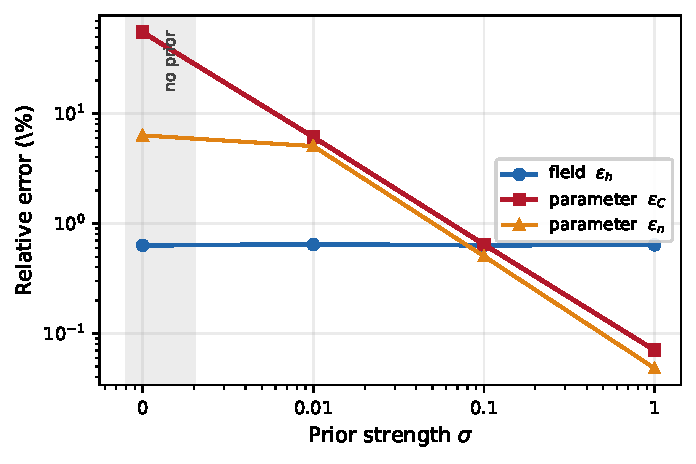
\includegraphics[width=0.60\textwidth]{figures/fig_identifiability.pdf}
\caption{Prior-strength study (ReLoBRaLo, prior balanced). The field error is
flat across four orders of magnitude of prior strength, while both parameter
errors fall steeply with it. The field is therefore fixed by the data and the
parameters by the prior; with no prior ($\sigma = 0$) the drainage coefficient
is unidentified to within a factor of two.}
\label{fig:ident}
\end{figure} With no prior at all the drainage coefficient is off by $54.99\%$, so
the data alone does not identify it --- unsurprising, since the drainage
depression is only $\sim 1\%$ of the water depth, and a $20\%$ change in $C$
moves $h$ by roughly $0.2\%$, below the $0.5\%$ observation noise.

The practical reading is that this inverse problem is only weakly identified,
and the prior is doing the identification. The choice of balancer then decides
the answer: over the configurations studied, $\epsilon_C$ ranges from
$0.001\%$ to $54.99\%$ depending on how the balancer treats a single loss
term. This is the strongest argument for the diagnostic and the wrapper: in a
weakly identified problem one cannot rely on the training loss to reveal that
a prior has been silently discarded.

\subsection{Repairing the Failures}

Figure~\ref{fig:fix} summarises the effect of the wrapper. For LL-EMA it
raises the prior weight from $1.6\times10^{-5}$ to $1.0$ and reduces the
drainage-coefficient error from $52.9\%$ to $0.030\%$. For LRA it bounds the
weight that previously reached $3.3\times10^7$.

\begin{figure}[t]
\centering
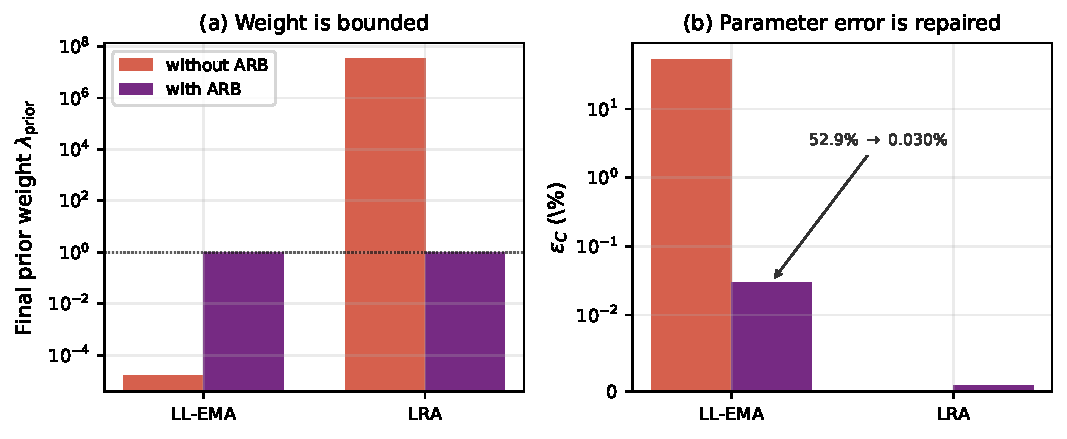
\includegraphics[width=0.95\textwidth]{figures/fig_fix.pdf}
\caption{Effect of the anchor-robust wrapper, which was given no information
about which loss is decoupled. (a) The prior weight is bounded at one for both
gradient-norm balancers. (b) The parameter error of LL-EMA falls from $52.9\%$
to $0.030\%$; LRA's apparent accuracy without the wrapper is the circular
result discussed in the text, not a successful inference.}
\label{fig:fix}
\end{figure} In both cases the field error is unchanged to within the
spread of the baseline runs ($0.680\%$ and $0.839\%$ versus $0.632\%$ and
$0.708\%$), confirming that the wrapper alters only the treatment of the
decoupled loss.

\subsection{Multi-Seed Robustness}

Table~\ref{tab:multiseed} reports the mean and standard deviation over three
seeds for the un-repaired configurations with the prior fixed, to establish
that the baseline behaviour is stable.

\begin{table}[t]
\centering
\caption{Multi-seed statistics over seeds $0,1,2$ (prior fixed, errors in \%).}
\label{tab:multiseed}
\begin{tabular}{lccc}
\toprule
Configuration & $\epsilon_h$ & $\epsilon_n$ & $\epsilon_C$ \\
\midrule
No balancing       & $0.549 \pm 0.012$ & $0.054 \pm 0.005$ & $0.067$ \\
LL-EMA             & $0.592 \pm 0.018$ & $0.041 \pm 0.001$ & $0.039$ \\
Causal weighting   & $0.919 \pm 0.007$ & $1.669 \pm 0.005$ & $2.814$ \\
LL-EMA + causal    & $1.216 \pm 0.016$ & $2.535 \pm 0.071$ & $3.276$ \\
\bottomrule
\end{tabular}
\end{table}

Standard deviations are small (below $3\%$ relative for $\epsilon_h$), so the
qualitative behaviour reported above is not a seed artefact.

\subsection{Generalisation to Another PDE}

To check that the mechanism is not specific to the shallow-water problem we
repeat the comparison on the 2D Navier--Stokes cylinder wake at
$\mathrm{Re}=100$, using the CFD data of \cite{raissi2019physics}. This is a
\emph{forward} problem: the loss consists of a PDE residual and a data misfit
only, and there is no parameter prior, so the decoupling mechanism of
Proposition~\ref{prop:decoupling} is absent by construction. The point of the
comparison is therefore to confirm that the wrapper does not disturb ordinary
balancing when no loss is decoupled.

\begin{table}[t]
\centering
\caption{Relative $L_2$ error on the Navier--Stokes cylinder wake
($8{,}000$ epochs) at the final time.}
\label{tab:ns}
\begin{tabular}{lcc}
\toprule
Configuration & $\epsilon_u$ & $\epsilon_v$ \\
\midrule
No balancing & $\mathbf{5.52\times10^{-2}}$ & $\mathbf{2.06\times10^{-1}}$ \\
LL-EMA & $6.80\times10^{-2}$ & $2.51\times10^{-1}$ \\
Causal weighting & $1.49\times10^{-1}$ & $6.53\times10^{-1}$ \\
Both & $1.93\times10^{-1}$ & $9.81\times10^{-1}$ \\
\bottomrule
\end{tabular}
\end{table}

With no decoupled loss the balancers behave conventionally: the un-balanced
baseline is best on both velocity components, and balancing gives no
improvement. This is consistent with the view that adaptive balancing helps
when there is genuine multi-task tension to resolve and is at best neutral
otherwise; it also confirms that the wrapper is inert when nothing is
decoupled, since it acts only on losses flagged by the diagnostic. Causal
weighting degrades the result, which we report for completeness; it is a
separate mechanism from the per-loss balancing studied here.

% ======================================================================
\section{Discussion}
% ======================================================================

\textbf{What the diagnostic is for.} The failures analysed here are silent by
construction: the balancer receives a zero, acts on it, and reports nothing.
The coupling ratio \eqref{eq:coupling} makes them visible at negligible cost.
We suggest reporting $c_k$ alongside loss weights whenever a balancer is used
with a heterogeneous loss set, and in particular whenever a loss depends on
parameters that are disjoint from the network --- as parameter priors do.

\textbf{Why a wrapper rather than a new balancer.} The failure is a property
of the anchor, not of the update rule, so it cannot be fixed by changing how
the weights are computed. Any balancer of the family \eqref{eq:balancer_family}
can be wrapped, which means existing pipelines can be made safe without being
replaced. The wrapper also leaves the visible losses' weights exactly as the
base method would have produced them.

\textbf{Weakly identified inverse problems.} The identifiability study
(\S\ref{sec:identifiability}) is a caution that goes beyond loss balancing. In
this problem the data does not identify the drainage coefficient, so the
recovered parameters are prior-determined, and the reported parameter error
measures the prior, not the inference. We would encourage reporting a
prior-perturbation check --- refit with a displaced prior centre and see
whether the parameters follow --- before interpreting parameter errors as
evidence of successful inference. That check is what revealed the issue here.

\textbf{Limitations.} (1) Our identifiability conclusion is specific to the
shallow-water problem and its observation operator; a problem with a stronger
parameter signature in the data may be well identified, in which case a
discarded prior is less damaging (although the diagnostic still applies). (2)
Whether the weak identifiability is partly an artefact of network capacity ---
a flexible network can absorb parameter error into the field --- is an open
question that a more constrained architecture might settle. (3) We study a
single base balancer per family; the two failure directions are however
properties of the functional forms, not of particular implementations.

% ======================================================================
\section{Conclusion}
% ======================================================================

Gradient-norm loss balancers estimate each loss's magnitude from its gradient
with respect to an anchor. When a loss is decoupled from that anchor the
estimate is zero, and we have shown that the resulting failure has two
directions fixed by the balancer's functional form: relative-norm balancers
switch the loss off, inverse-ratio balancers let it dominate. Neither is
reported by the training loss. We introduced the anchor-coupling ratio to
detect the situation, and an anchor-robust wrapper that corrects it for any
base balancer without manual intervention, reducing a $52.9\%$ parameter error
to $0.030\%$ and bounding a weight that had reached $3.3\times10^7$. Because
parameter priors in inverse problems are exactly the decoupled case, and
because such problems are often only weakly identified, we argue that the
diagnostic should be part of the default toolkit when PINNs are used for
parameter inference.

% ======================================================================
\section*{Declaration of Competing Interest}
% ======================================================================

The author declares that he has no known competing financial interests or
personal relationships that could have appeared to influence the work reported
in this paper.

% ======================================================================
\section*{Data and Code Availability}
% ======================================================================

Source code, including the finite-volume reference solver, all balancer
implementations, the diagnostic and the anchor-robust wrapper, is available at
\url{https://github.com/YuhaoPeng1103/ca-pinn}.

% ======================================================================
\section*{Declaration of generative AI and AI-assisted technologies in the writing process}
% ======================================================================

During the preparation of this work the author used generative AI tools to
assist with code implementation and debugging, and to draft and polish
portions of the manuscript. All AI-assisted code was tested against analytical
or numerically verified reference solutions, and all AI-assisted text was
reviewed and edited by the author, who takes full responsibility for the
content of the publication.

% ======================================================================
\section*{Acknowledgments}
% ======================================================================

The author acknowledges the foundational PINN codebase by Maziar Raissi et al.

% ======================================================================
\bibliographystyle{elsarticle-num}
\bibliography{references}

\end{document}
